\documentclass{article}[18pt]
\ProvidesPackage{format}
%Page setup
\usepackage[utf8]{inputenc}
\usepackage[margin=0.7in]{geometry}
\usepackage{parselines} 
\usepackage[english]{babel}
\usepackage{fancyhdr}
\usepackage{titlesec}
\hyphenpenalty=10000

\pagestyle{fancy}
\fancyhf{}
\rhead{Sam Robbins}
\rfoot{Page \thepage}

%Characters
\usepackage{amsmath}
\usepackage{amssymb}
\usepackage{gensymb}
\newcommand{\R}{\mathbb{R}}

%Diagrams
\usepackage{pgfplots}
\usepackage{graphicx}
\usepackage{tabularx}
\usepackage{relsize}
\pgfplotsset{width=10cm,compat=1.9}
\usepackage{float}

%Length Setting
\titlespacing\section{0pt}{14pt plus 4pt minus 2pt}{0pt plus 2pt minus 2pt}
\newlength\tindent
\setlength{\tindent}{\parindent}
\setlength{\parindent}{0pt}
\renewcommand{\indent}{\hspace*{\tindent}}

%Programming Font
\usepackage{courier}
\usepackage{listings}
\usepackage{pxfonts}

%Lists
\usepackage{enumerate}
\usepackage{enumitem}

% Networks Macro
\usepackage{tikz}


% Commands for files converted using pandoc
\providecommand{\tightlist}{%
	\setlength{\itemsep}{0pt}\setlength{\parskip}{0pt}}
\usepackage{hyperref}

% Get nice commands for floor and ceil
\usepackage{mathtools}
\DeclarePairedDelimiter{\ceil}{\lceil}{\rceil}
\DeclarePairedDelimiter{\floor}{\lfloor}{\rfloor}

% Allow itemize to go up to 20 levels deep (just change the number if you need more you madman)
\usepackage{enumitem}
\setlistdepth{20}
\renewlist{itemize}{itemize}{20}

% initially, use dots for all levels
\setlist[itemize]{label=$\cdot$}

% customize the first 3 levels
\setlist[itemize,1]{label=\textbullet}
\setlist[itemize,2]{label=--}
\setlist[itemize,3]{label=*}

% Definition and Important Stuff
% Important stuff
\usepackage[framemethod=TikZ]{mdframed}

\newcounter{theo}[section]\setcounter{theo}{0}
\renewcommand{\thetheo}{\arabic{section}.\arabic{theo}}
\newenvironment{important}[1][]{%
	\refstepcounter{theo}%
	\ifstrempty{#1}%
	{\mdfsetup{%
			frametitle={%
				\tikz[baseline=(current bounding box.east),outer sep=0pt]
				\node[anchor=east,rectangle,fill=red!50]
				{\strut Important};}}
	}%
	{\mdfsetup{%
			frametitle={%
				\tikz[baseline=(current bounding box.east),outer sep=0pt]
				\node[anchor=east,rectangle,fill=red!50]
				{\strut Important:~#1};}}%
	}%
	\mdfsetup{innertopmargin=10pt,linecolor=red!50,%
		linewidth=2pt,topline=true,%
		frametitleaboveskip=\dimexpr-\ht\strutbox\relax
	}
	\begin{mdframed}[]\relax%
		\centering
		}{\end{mdframed}}



\newcounter{lem}[section]\setcounter{lem}{0}
\renewcommand{\thelem}{\arabic{section}.\arabic{lem}}
\newenvironment{defin}[1][]{%
	\refstepcounter{lem}%
	\ifstrempty{#1}%
	{\mdfsetup{%
			frametitle={%
				\tikz[baseline=(current bounding box.east),outer sep=0pt]
				\node[anchor=east,rectangle,fill=blue!20]
				{\strut Definition};}}
	}%
	{\mdfsetup{%
			frametitle={%
				\tikz[baseline=(current bounding box.east),outer sep=0pt]
				\node[anchor=east,rectangle,fill=blue!20]
				{\strut Definition:~#1};}}%
	}%
	\mdfsetup{innertopmargin=10pt,linecolor=blue!20,%
		linewidth=2pt,topline=true,%
		frametitleaboveskip=\dimexpr-\ht\strutbox\relax
	}
	\begin{mdframed}[]\relax%
		\centering
		}{\end{mdframed}}
\lhead{Theory of Computation - Algorithms and Complexity}
\newtheorem{theorem}{Theorem}

\begin{document}
\begin{center}
\underline{\huge NP-Completeness}
\end{center}
\section{Polynomial time reductions}
Problem X polynomially reduces to problem Y if an arbitrary instance of problem X can be
\begin{itemize}
	\item Transformed to an instance of problem Y in a polynomial number of steps and then
	\item Solved using a polynomial number of calls to an oracle that solve problem Y
\end{itemize}
Notation: X is polynomial time reducible to Y is written as $X\leqslant Y$\\
\\
If $X\leqslant Y$ and $Y\leqslant X$, then X and Y are equivalent
\section{NP completeness proofs}
To prove that a problem $\Pi$ is NP complete we now have to perform two steps
\begin{enumerate}
	\item Show that $\Pi$ belongs to NP
	\item Find a known NP complete problem and show $\Pi'\leqslant \Pi$
\end{enumerate}
If we can complete step 2 but not step 1, then we say that $\Pi$ is NP hard
\section{Proof techniques}
Restriction
\begin{itemize}
	\item Show that $\Pi'$ is a subproblem of $\Pi$
\end{itemize}
Local replacement
\begin{itemize}
	\item Show that every basic unit in an instance of $\Pi'$ can be replaced by a different structure in a uniform way to obtain an instance of $\Pi$
\end{itemize}
Component design
\begin{itemize}
	\item Show that the constituents of an instance of $\Pi$ can be used to "design" components that can be combined to "realise" instanced of $\Pi'$
\end{itemize}
\section{NP completeness of vertex cover}
\begin{problem}[Vertex cover]
\textbf{Instance} - A graph G=(V,E), and a natural number k\\
\textbf{Question} - Is there a set $W\subseteq V$, which $|W|\leqslant k$, such that for each edge $(i,j)\in E$
$$\{i,j\}\cap W\neq \varnothing$$
\end{problem}
To show that Vertex Cover is NP complete we shall reduce satisfiability to vertex cover\\
\\
Given a formula f with n variables and clauses $C_1,C_2,...,C_m$
\begin{itemize}
	\item For each variable x create two adjacent vertices $x^t$ and $x^f$ to represent the literals $x$ and $\lnot x$
	\item For each clause $C_j$ of size $n_j$ create a complete subgraph $G_j$ with vertices connected to corresponding literals
	\item Set $k=n+\sum_{j=1}^{m}(n_j-1)$
\end{itemize}
\begin{theorem}
There exists a truth assignment that satisfies the formula f iff there exists a vertex cover of the constructed graph with size at most k
\end{theorem}
\textbf{Proof} in $\Rightarrow$ direction
\begin{itemize}
	\item At least one of each pair $(x^f,x^t)$ must be in the cover
	\item At least $n_j-1$ vertices from each complete graph $G_j$ must be in the cover
	\item If the formula is satisfiable, then choose the cover by choosing each literal assigned True plus all but one vertex in each $G_j$ (omit a vertex which is connected to a satisfied literal)
\end{itemize}
Proof in $\Leftarrow$ direction
\begin{itemize}
	\item If a vertex cover exists, assign each boolean variable according to whether $x^t$ or $x^f$ is in M
	\item By the choice of k, there must be exactly one vertex in each clique which is not in M. This vertex must be adjacent to a literal-vertex in M, hence clause is satisfied.
\end{itemize}
\section{NP completeness of clique}
\begin{problem}[Clique]
\textbf{Instance} - A finite graph $G=(V,E)$ and an integer k\\
\textbf{Question} - Does G have a clique of size k?
\end{problem}
A set of vertices W is a vertex cover in G iff V-W is a clique in the complement of G
\section{NP completeness of Hitting Set}
\begin{problem}[Hitting Set]
\textbf{Instance} - Collection C of subsets of a set S and a positive integer k\\
\textbf{Question} - Does S contain a hitting set for C of size k or less. i.e. a subset $S'\subseteq S$ with $|S'|\leqslant k$ such that $S'$ contains at least one element from each subset from C 
\end{problem}
To show that Hitting Set is NP complete restrict it to instances with $|c|=2$ for all $c\in C$ and you get vertex cover
\section{3 Satisfiability}
To show that 3 satisfiability is NP complete we reduce Satisfiability to 3-Satisfiability\\
\\
Proof\\
Replace every clause
$$C=x_1\lor x_2 \lor ... \lor x_k$$
with $k>3$ by:
$$C'=(x_1\lor x_2 \lor y_1) \land (\lnot y_1 \lor x_3 \lor y_2) \lor ... \lor (\lnot y_{k-3} \lor x_{k-1} \lor x_k)$$
C is satisfiable iff C' is, since at least one of the literals other than the y's must be true
\section{NP completeness of Graph 3 colouring}
\begin{problem}[Graph 3-Colouring]
\textbf{Instance} - A graph G=(V,E)\\
\textbf{Question} - Is there a colouring of the vertices of G in 3 colours such that adjacent vertices are all different colours
\end{problem}
To show completeness, reduce 3 satisfiability to graph 3 colouring
\section{Encoding}
Given a 3CNF formula f, encode it as a graph $G_f$ such that the graph has a (proper) 3 colouring iff the formula is satisfiable
\begin{itemize}
	\item Lets introduce 3 colours: ground, true and false
	\item Introduce a 3-clique of designated vertices, $v_g$, $v_t$ and $v_f$. By symmetry, assume without loss of generality that they are always coloured ground, true and false, respectively
	\item For each variable x, introduce two vertices $x_p$ and $x_n$ (for $x$ and $\lnot x$), and add all edges between $x_p$, $x_n$ and $v_g$. Hence one of $x_p$ and $x_n$ must be true and the other false
	\item For each clause C, say $C=(x\lor \lnot y \lor z)$ connect vertices $x_p$,$y_n$ and $z_p$ via the below gadget consisting of five clauses vertices which we call the C-vertices
\end{itemize}
\begin{center}
	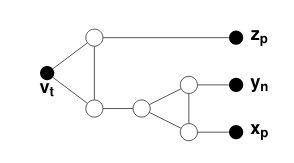
\includegraphics[scale=0.7]{gadget}
\end{center}
\subsection{Proof}
First suppose that $G_f$ has a 3-colouring c
\begin{itemize}
	\item As $v_g$, $v_t$ $v_f$ form a triangle, we may assume without loss of generality that $c(v_g)-1$, $c(v_t)=2$ and $c(v_f)=3$
	\item For every variable $x$, $c(x_p)\in \{2,3\}$ and $c(x_n)\in \{2,3\}$, as $x_p$ and $x_n$ are both adjacent to $v_g$
	\item As $x_p$ and $x_n$ are adjacent, this means that if $c(x_p)=2$ then $c(x_n)=3$ and vice versa
	\item Let $\tau$ be the truth assignment of f that set x to be True if $c(x_p)=2$ and false if it equals 3
	\item We claim that $\tau$ is satisfying. Suppose not and C is a clause whose three literals $\ell_1,\ell_2$ and $\ell_3$ are all false.
	\begin{itemize}
		\item Without loss of generality, let $C=(x\lor \lnot y \lor z)$
		\item Then $c(x_p)=c(y_n)=c(z_p)=3$
		\item As $c(v_t)=1$, the C-vertex adjacent to $z_p$ has colour 2, which means that it's C-neighbour has colour 3
		\item But now as $c(x_p)=c(y_n)=3$, the tree remaining C-vertices all have colour 1 or 2. As they form a triangle this is a contradiction as c is a 3-colouring of $G_f$
	\end{itemize}
\end{itemize}
Now suppose that f has a satisfying truth assignment $\tau$. We define a mapping c as follows
\begin{itemize}
	\item Set $c(v_g)=1$, $c(v_t)=2$ and $c(v_f)=3$
	\item If x is True, then set $c(x_p)=2$ and $c(x_n)=3$ and vice versa for False
	\item For every clause C do as follows
	\begin{itemize}
		\item Without loss of generality, let $C=(x\lor\lnot y\lor z)$ As $\tau$ is satisfying, at least one of $x,\lnot y$ or $z$ is True.
		\item This means that at least one of $x_p,y_n,z_p$ gets colour 2. Then we can colour the five C-vertices with colours 1,2,3 in such a way that no two adjacent vertices are coloured alike
	\end{itemize}
	\item From above we conclude that c is a 3-colouring of $G_f$
\end{itemize}


\end{document}